\documentclass[11pt, a4paper, plain]{article}

\usepackage{fontspec}
\usepackage{inputenc}
\usepackage[czech]{babel}
\usepackage{luavlna}
\usepackage{graphicx}
\usepackage{tabularx}
\usepackage{array}
\usepackage[bookmarksopen,colorlinks,plainpages=false,linkcolor=black,urlcolor=blue,citecolor=black,filecolor=black,menucolor=black,unicode=true,breaklinks]{hyperref}
\usepackage{csquotes}
\usepackage{caption}
\usepackage{parskip}
\usepackage[margin=2.5cm, bindingoffset=1cm]{geometry}
\usepackage{titlesec}
\usepackage{lipsum}
\usepackage{todonotes}
\usepackage{csquotes}
\usepackage{latexcolors}
\usepackage{minted}
\usepackage{algorithm}
\usepackage{algpseudocode}
\usepackage{etoolbox}
\usepackage{amsmath}
\usepackage{booktabs}
\usepackage{colortbl}
\usepackage{siunitx}
\usepackage{svg}
\usepackage{tocloft}
\usepackage{bookmark}
\usepackage{subcaption}
\usepackage{enumitem}
\usepackage{amssymb}
\usepackage{unicode-math}
\usepackage{tabularx}
\usepackage{multirow}
\usepackage{hologo}

\setmainfont{Linux Biolinum G}
\setmonofont{Inconsolata}[Scale=0.925]
\setmathfont{Libertinus Math}

\setlength{\intextsep}{5mm} % nastavení mezery okolo obrázků
\setlength{\marginparwidth}{2cm}
\marginparsep=15pt
\linespread{1.3}
\unitlength=1mm % nastavení volby jednotek

% Use squares instead of circles
\setlist[itemize]{label = \raisebox{0.2ex}{\tiny$\blacksquare$}}

% Define not variants of if and while
\algnewcommand\algorithmicnot{\textbf{not}}
\algdef{SE}[IF]{IfNot}{EndIf}[1]{\algorithmicif\ \algorithmicnot\ #1\ \algorithmicthen}{\algorithmicend\ \algorithmicif}
\algdef{SE}[WHILE]{WhileNot}{EndWhile}[1]{\algorithmicwhile\ \algorithmicnot\ #1\ \algorithmicthen}{\algorithmicend\ \algorithmicwhile}

% Use default font for algorithmic
% \AtBeginEnvironment{algorithmic}{\rmfamily}

% Left-justified comment
\algnewcommand{\LeftComment}[1]{\Statex \(\triangleright\) #1}

% \usemintedstyle{tango}
\setminted{
    style=tango,
    bgcolor=ghostwhite,
    fontsize=\footnotesize,
    frame=none,
}

\AtBeginEnvironment{minted}{\linespread{0.3}}

% Use comma instead of period (czech standard)
\sisetup{locale = DE}

% List of attachments
\newcommand{\listappendixname}{Seznam příloh}
\newlistof{myappendices}{app}{\listappendixname}

% Tímto vypneš číslování stránek pouze pro tento seznam
\cftpagenumbersoff{myappendices}

% Příkaz pro přidání položky do seznamu příloh
\newcommand{\addextappendix}[1]{%
  \addcontentsline{app}{myappendices}{#1}
}

\begin{document}

\section*{Příloha F -- Podrobný popis funkčností SD karty}

Tato kapitola dokumentuje návrh a implementaci vstupně-výstupní vrstvy určené pro komunikaci se SD
kartou prostřednictvím sběrnice SPI na mikrokontroléru RP2350. Cílem bylo vytvoření
spolehlivého abstrakčního rozhraní mezi hardwarovými periferiemi a souborovým systémem
\textbf{FatFs}, jenž ke svému běhu vyžaduje standardizovaný blokový přístup k úložnému médiu.

Navržené řešení je strukturováno do několika logických úrovní. Tento přístup odděluje hardwarově
závislé části kódu od vyšší aplikační logiky, čímž je zajištěna modularita a vysoká míra
přenositelnosti (portability) případné implementace na jiné platformy.

\subsection{Architektura řešení}

Z hlediska softwarové architektury je systém dekomponován do tří základních vrstev:

\begin{itemize}
    \item Hardwarová vrstva (platform layer)
    \item Ovladač SD karty (storage layer)
    \item Disk I/O rozhraní pro FatFs (disk I/O layer)
\end{itemize}

Tato struktura definuje jasné hranice odpovědnosti pro jednotlivé části systému a značně usnadňuje
případné budoucí rozšiřování či údržbu kódu.

\subsection{Inicializace SD karty}

\begin{figure}[htbp]
    \centering
    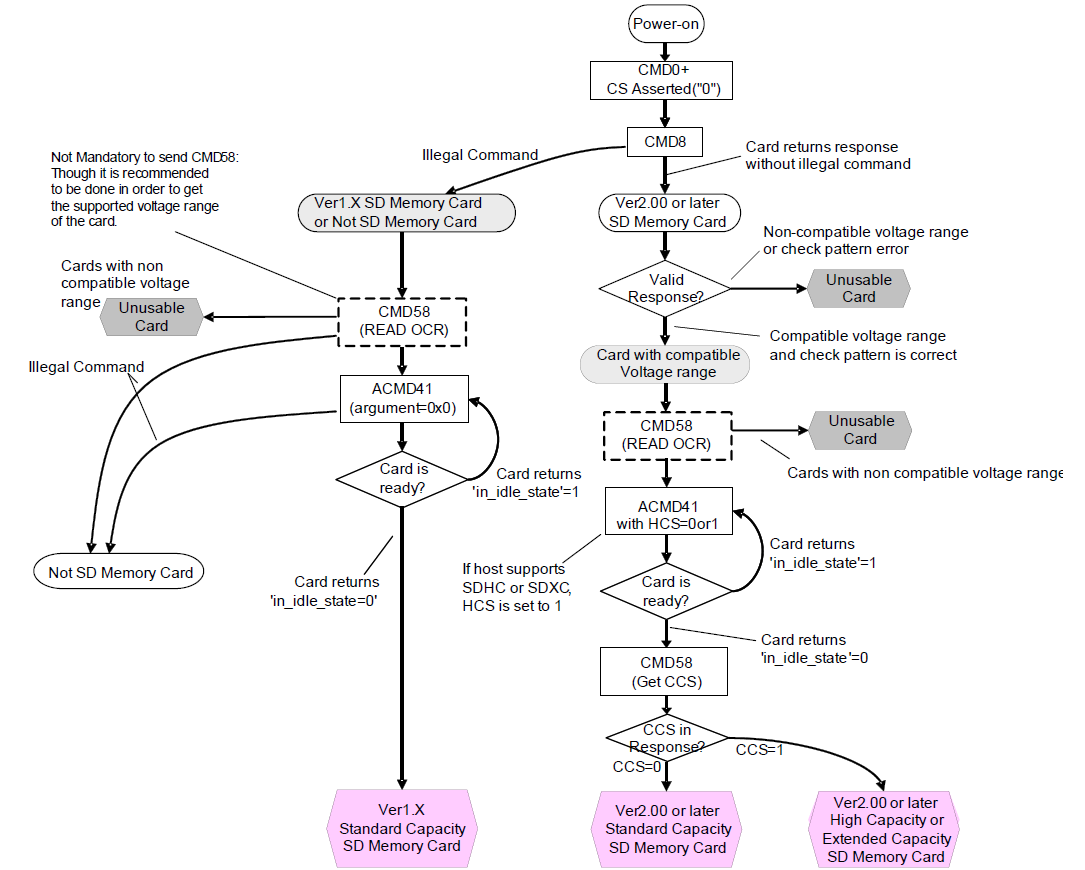
\includegraphics[width=\textwidth]{../../images/sd_init.png}
    \caption{Inicializační sekvence SD karty. Zdroj [16].}
    \label{fig:motherboard}
\end{figure}

Proces inicializace SD karty probíhá ve standardním režimu SPI a striktně dodržuje sekvenci
definovanou specifikací fyzické vrstvy SD karet (viz [16]). Po prvotním nastavení sběrnice
SPI na nízkou přenosovou rychlost je karta uvedena do definovaného výchozího stavu pomocí série
hodinových impulsů při záměrně deaktivovaném signálu \textbf{CS} (Chip Select).

Následně je opakovaně odesílán příkaz \textbf{CMD0}, jehož účelem je softwarový reset a přepnutí
karty do stavu \textit{IDLE}. Vzhledem k technologickým prodlevám nemusí být odpověď karty okamžitě
validní, proto je implementován robustní mechanismus dotazování s omezeným počtem pokusů (timeout).

Po úspěšném přechodu do stavu \textit{IDLE} je prostřednictvím příkazu \textbf{CMD8} ověřena
kompatibilita karty se specifikací SD verze 2.0 a novější. Validní odpověď formátu R7 zároveň slouží
k potvrzení podporovaného napěťového rozsahu.

Samotná inicializace média pokračuje specifickou sekvencí příkazů \textbf{CMD55} a \textbf{ACMD41},
přičemž pro podporu moderních paměťových médií je v argumentu aktivován příznak \textit{HCS} (High
Capacity Support). Jakmile je inicializační smyčka úspěšně ukončena, provede se vyčtení registru OCR
pomocí příkazu \textbf{CMD58}. Na základě obsahu tohoto registru je identifikován typ vložené karty
(\textbf{SDSC} nebo \textbf{SDHC/SDXC}), což je klíčový parametr pro správný výpočet adresace
fyzických sektorů.

V závěrečné fázi inicializace je komunikační rozhraní SPI přepnuto na maximální podporovanou
přenosovou rychlost pro efektivní provoz.

\subsection{Hardwarová vrstva (platform layer)}

Hardwarově závislá vrstva plní funkci abstrakce mikrokontroléru. Zajišťuje přímou obsluhu periferií,
konktrétně SPI řadiče, sdílených datových linek a vyhrazených GPIO pinů. Součástí této vrstvy je
rovněž správa elementárního časování komunikace.

Poskytované funkční rozhraní zahrnuje:

\begin{itemize}
    \item Obousměrný přenos jednotlivých bytů po sběrnici SPI.
    \item Dynamické řízení přenosové rychlosti hodin (SCLK).
    \item Ovládání signálu \textbf{Chip Select (CS)}.
    \item Nízkoúrovňovou inicializaci SPI periferie.
    \item Generování deterministických časových prodlev (delay).
\end{itemize}

Tato vrstva jako jediná přímo interaguje s registry mikrokontroléru RP2350 a je plně platformně
závislá.

\subsection{Ovladač SD karty (storage layer)}

Vrstva ovladače implementuje vlastní komunikační protokol SD karty nad sběrnicí SPI a ke své
činnosti využívá služby poskytované hardwarovou vrstvou.

Mezi primární zodpovědnosti modulu patří:

\begin{itemize}
    \item Exekuce inicializační sekvence (\textbf{CMD0}, \textbf{CMD8}, \textbf{ACMD41},
        \textbf{CMD58}).
    \item Detekce a správa typu paměťového média (SDSC, SDHC).
    \item Realizace blokového čtení dat (\textbf{CMD17}).
    \item Realizace blokového zápisu dat (\textbf{CMD24}).
    \item Translace logických adres na fyzické adresy sektorů.
    \item Validace datových tokenů a zpracování stavových kódů (R1, R2, R7 odpovědi).
\end{itemize}

V kontextu implementovaného systému je SD karta reprezentována jako unifikované blokové zařízení s
pevnou velikostí alokační jednotky (sektoru) 512 bytů.

Během operace čtení odesílá karta – po úspěšném přijetí a zpracování příkazu – datový token
\texttt{0xFE}, který mikroprocesoru signalizuje připravenost k přesunu dat. Bezprostředně poté
následuje přenos samotného bloku o velikosti 512 bytů a dvou kontrolních bytů CRC. Tyto
byty jsou v rámci této implementace vyčteny a následně zahozeny, neboť striktní CRC kontrola
komunikace je v režimu SPI specifikací definována jako volitelná.

Během operace zápisu odpovídá karta po přijetí kompletního datového bloku stavovým tokenem (data
response token), ze kterého lze dekódovat úspěšnost uložení. Interní proces zápisu dat do flash
paměti karty je následně signalizován držením datové linky v logické nule (busy state) a ukončen
jejím uvolněním.

\subsection{I/O rozhraní pro FatFs (disk I/O layer)}

Vrstva diskového I/O rozhraní slouží jako propojovací prvek (wrapper) mezi nízkoúrovňovým
ovladačem SD karty a nezávislým modulem souborového systému \textbf{FatFs}. Samotná knihovna FatFs
je striktně hardwarově agnostická a vyžaduje implementaci sady definovaných blokových operací.

Tato mezivrstva poskytuje a mapuje následující systémová volání:

\begin{itemize}
    \item \texttt{disk\_initialize()} – provedení inicializační sekvence média.
    \item \texttt{disk\_status()} – zjištění aktuálního stavu disku (inicializován, chybí, chráněn proti zápisu).
    \item \texttt{disk\_read()} – čtení $N$ sektorů dat.
    \item \texttt{disk\_write()} – zápis $N$ sektorů dat.
\end{itemize}

Uvedené funkce efektivně překládají unifikované požadavky souborového systému na sérii specifických
příkazů ovladače SD karty. Z pohledu aplikačního rozhraní knihovny FatFs se SD karta
jeví jako transparentní úložné zařízení a veškeré detaily týkající se sériové SPI komunikace
zůstávají skryté na nižších vrstvách abstrakce.

\end{document}
